\begin{figure}[!htb]
  \centering
  \begin{subfigure}[b]{0.45\textwidth}
    \caption*{Squared Exponential Kernel}
  \end{subfigure}
  \begin{subfigure}[b]{0.45\textwidth}
    \caption*{Exponential Kernel}
  \end{subfigure}

  \begin{subfigure}[b]{0.15\textwidth}
    \caption*{$\Gc^*$}
    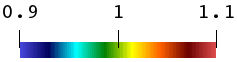
\includegraphics[width=\textwidth]{Chapter4/figures/rainbow_horizontal.png}
  \end{subfigure}
  \begin{subfigure}[b]{0.15\textwidth}
    \caption*{$\psi_c^*$}
    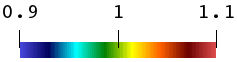
\includegraphics[width=\textwidth]{Chapter4/figures/rainbow_horizontal.png}
  \end{subfigure}
  \begin{subfigure}[b]{0.15\textwidth}
    \caption*{$d$}
    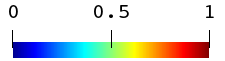
\includegraphics[width=\textwidth]{Chapter4/figures/jet_horizontal.png}
  \end{subfigure}
  \begin{subfigure}[b]{0.15\textwidth}
    \caption*{$\Gc^*$}
    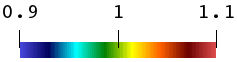
\includegraphics[width=\textwidth]{Chapter4/figures/rainbow_horizontal.png}
  \end{subfigure}
  \begin{subfigure}[b]{0.15\textwidth}
    \caption*{$\psi_c^*$}
    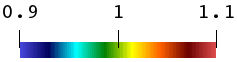
\includegraphics[width=\textwidth]{Chapter4/figures/rainbow_horizontal.png}
  \end{subfigure}
  \begin{subfigure}[b]{0.15\textwidth}
    \caption*{$d$}
    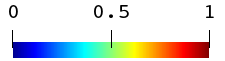
\includegraphics[width=\textwidth]{Chapter4/figures/jet_horizontal.png}
  \end{subfigure}

  \begin{subfigure}[b]{0.15\textwidth}
    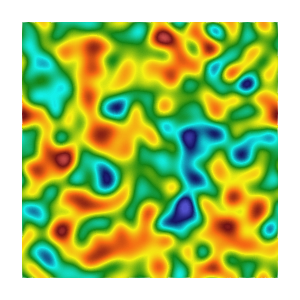
\includegraphics[width=\textwidth]{Chapter4/figures/2D/Gc_sqexp_cartesian_5_5_rho_0_seed_c.png}
    \caption{}
    \label{fig: Chapter4/2D/Gc_sqexp_cartesian_5_5_rho_0_seed_c}
  \end{subfigure}
  \begin{subfigure}[b]{0.15\textwidth}
    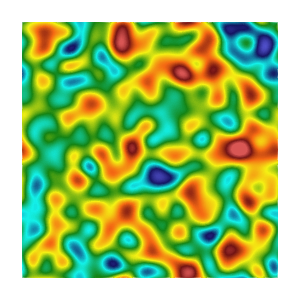
\includegraphics[width=\textwidth]{Chapter4/figures/2D/psic_sqexp_cartesian_5_5_rho_0_seed_c.png}
    \caption{}
    \label{fig: Chapter4/2D/psic_sqexp_cartesian_5_5_rho_0_seed_c}
  \end{subfigure}
  \begin{subfigure}[b]{0.15\textwidth}
    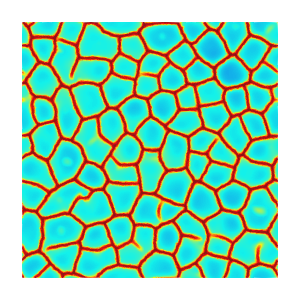
\includegraphics[width=\textwidth]{Chapter4/figures/2D/d_sqexp_cartesian_5_5_rho_0_seed_c.png}
    \caption{}
    \label{fig: Chapter4/2D/d_sqexp_cartesian_5_5_rho_0_seed_c}
  \end{subfigure}
  \begin{subfigure}[b]{0.15\textwidth}
    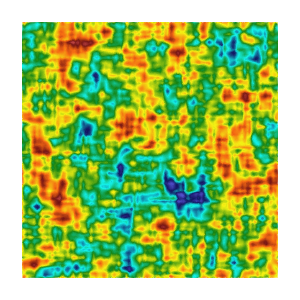
\includegraphics[width=\textwidth]{Chapter4/figures/2D/Gc_exp_cartesian_5_5_rho_0_seed_c.png}
    \caption{}
    \label{fig: Chapter4/2D/Gc_exp_cartesian_5_5_rho_0_seed_c}
  \end{subfigure}
  \begin{subfigure}[b]{0.15\textwidth}
    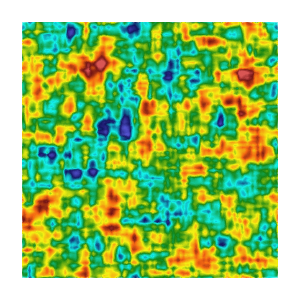
\includegraphics[width=\textwidth]{Chapter4/figures/2D/psic_exp_cartesian_5_5_rho_0_seed_c.png}
    \caption{}
    \label{fig: Chapter4/2D/psic_exp_cartesian_5_5_rho_0_seed_c}
  \end{subfigure}
  \begin{subfigure}[b]{0.15\textwidth}
    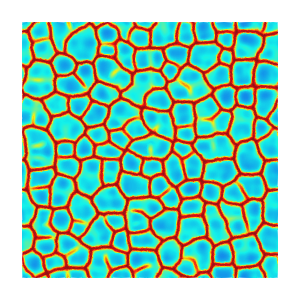
\includegraphics[width=\textwidth]{Chapter4/figures/2D/d_exp_cartesian_5_5_rho_0_seed_c.png}
    \caption{}
    \label{fig: Chapter4/2D/d_exp_cartesian_5_5_rho_0_seed_c}
  \end{subfigure}

  \begin{subfigure}[b]{0.15\textwidth}
    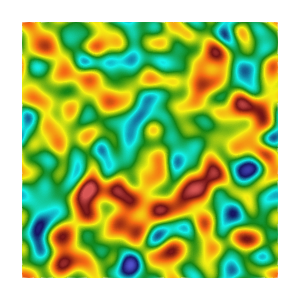
\includegraphics[width=\textwidth]{Chapter4/figures/2D/Gc_sqexp_cartesian_5_5_rho_0_seed_d.png}
    \caption{}
    \label{fig: Chapter4/2D/Gc_sqexp_cartesian_5_5_rho_0_seed_d}
  \end{subfigure}
  \begin{subfigure}[b]{0.15\textwidth}
    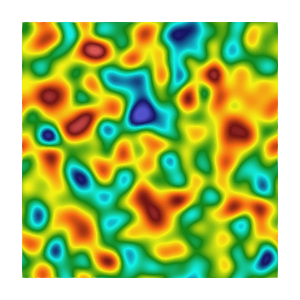
\includegraphics[width=\textwidth]{Chapter4/figures/2D/psic_sqexp_cartesian_5_5_rho_0_seed_d.png}
    \caption{}
    \label{fig: Chapter4/2D/psic_sqexp_cartesian_5_5_rho_0_seed_d}
  \end{subfigure}
  \begin{subfigure}[b]{0.15\textwidth}
    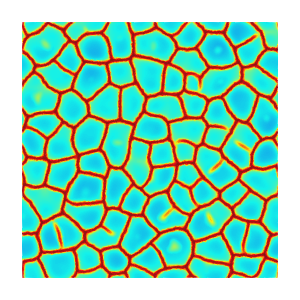
\includegraphics[width=\textwidth]{Chapter4/figures/2D/d_sqexp_cartesian_5_5_rho_0_seed_d.png}
    \caption{}
    \label{fig: Chapter4/2D/d_sqexp_cartesian_5_5_rho_0_seed_d}
  \end{subfigure}
  \begin{subfigure}[b]{0.15\textwidth}
    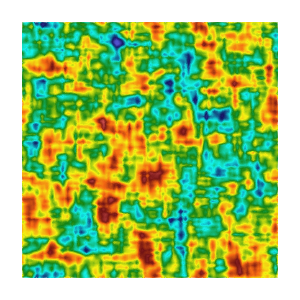
\includegraphics[width=\textwidth]{Chapter4/figures/2D/Gc_exp_cartesian_5_5_rho_0_seed_d.png}
    \caption{}
    \label{fig: Chapter4/2D/Gc_exp_cartesian_5_5_rho_0_seed_d}
  \end{subfigure}
  \begin{subfigure}[b]{0.15\textwidth}
    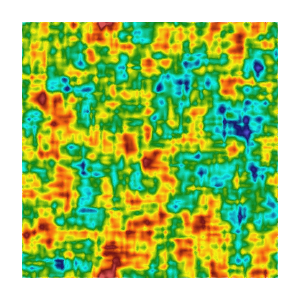
\includegraphics[width=\textwidth]{Chapter4/figures/2D/psic_exp_cartesian_5_5_rho_0_seed_d.png}
    \caption{}
    \label{fig: Chapter4/2D/psic_exp_cartesian_5_5_rho_0_seed_d}
  \end{subfigure}
  \begin{subfigure}[b]{0.15\textwidth}
    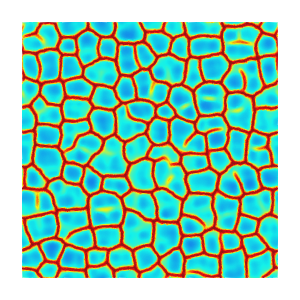
\includegraphics[width=\textwidth]{Chapter4/figures/2D/d_exp_cartesian_5_5_rho_0_seed_d.png}
    \caption{}
    \label{fig: Chapter4/2D/d_exp_cartesian_5_5_rho_0_seed_d}
  \end{subfigure}

  \begin{subfigure}[b]{0.15\textwidth}
    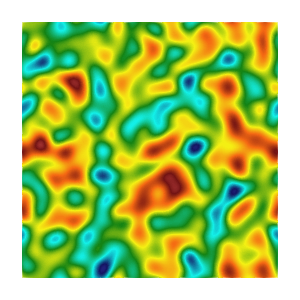
\includegraphics[width=\textwidth]{Chapter4/figures/2D/Gc_sqexp_cartesian_5_5_rho_0_seed_e.png}
    \caption{}
    \label{fig: Chapter4/2D/Gc_sqexp_cartesian_5_5_rho_0_seed_e}
  \end{subfigure}
  \begin{subfigure}[b]{0.15\textwidth}
    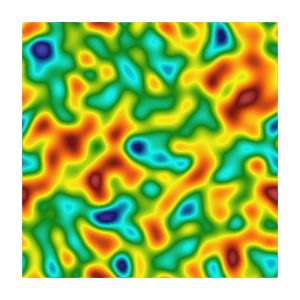
\includegraphics[width=\textwidth]{Chapter4/figures/2D/psic_sqexp_cartesian_5_5_rho_0_seed_e.png}
    \caption{}
    \label{fig: Chapter4/2D/psic_sqexp_cartesian_5_5_rho_0_seed_e}
  \end{subfigure}
  \begin{subfigure}[b]{0.15\textwidth}
    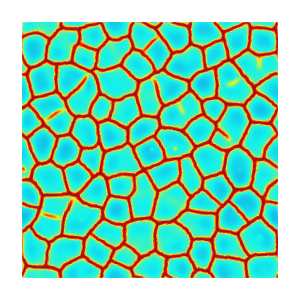
\includegraphics[width=\textwidth]{Chapter4/figures/2D/d_sqexp_cartesian_5_5_rho_0_seed_e.png}
    \caption{}
    \label{fig: Chapter4/2D/d_sqexp_cartesian_5_5_rho_0_seed_e}
  \end{subfigure}
  \begin{subfigure}[b]{0.15\textwidth}
    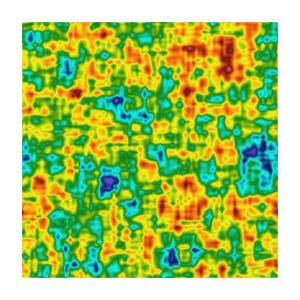
\includegraphics[width=\textwidth]{Chapter4/figures/2D/Gc_exp_cartesian_5_5_rho_0_seed_e.png}
    \caption{}
    \label{fig: Chapter4/2D/Gc_exp_cartesian_5_5_rho_0_seed_e}
  \end{subfigure}
  \begin{subfigure}[b]{0.15\textwidth}
    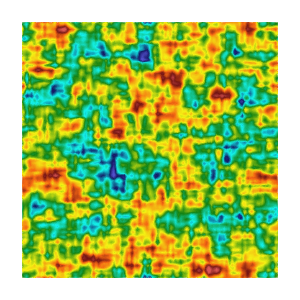
\includegraphics[width=\textwidth]{Chapter4/figures/2D/psic_exp_cartesian_5_5_rho_0_seed_e.png}
    \caption{}
    \label{fig: Chapter4/2D/psic_exp_cartesian_5_5_rho_0_seed_e}
  \end{subfigure}
  \begin{subfigure}[b]{0.15\textwidth}
    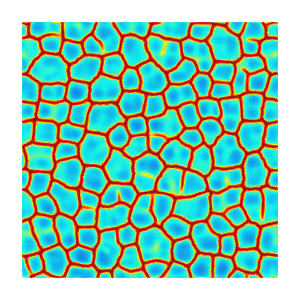
\includegraphics[width=\textwidth]{Chapter4/figures/2D/d_exp_cartesian_5_5_rho_0_seed_e.png}
    \caption{}
    \label{fig: Chapter4/2D/d_exp_cartesian_5_5_rho_0_seed_e}
  \end{subfigure}
  \caption{ Three pairs of qualitative comparison of smoothness of the kernel function with the same normalized  correlation length $L^* = 0.05$. (a-f) pair 1 (g-l) pair 2 (m-r) pair 3. Each row compares two kernel functions transformed from the same samples of the underlying Gaussian fields. }
  \label{fig: Chapter4/2D/compare_smoothness}
\end{figure}
